\chapter[Improving Deep Neural Networks]{Improving Deep Neural Networks\setcounter{footnote}{0}\footnote{Hyperparameter Tuning, Regularization and Optimization}}

%%%
\section{Setting up your ML application}

%%%%
\subsection{Train/dev/test sets}
对于数据集,我们通常将其分为三个部分:
\begin{itemize}
    \item \textbf{Training set}: 训练集,用于训练模型。一般占60\%。
    \item \textbf{Dev (development) set}: 开发集,用于调整模型的超参数。一般占20\%。
    \item \textbf{Test set}: 测试集,用于测试模型的性能。一般占20\%。
\end{itemize}
有时候,我们会将数据集仅分为训练集和开发集,而没有测试集。这时候,我们通常将二者的比例调整为70\%和30\%。

%%%%
\subsection{Bias and Variance}
\textbf{偏差(Bias)}描述了模型的预测值与真实值之间的差距。Bias越大,说明模型越不准确。
而\textbf{方差(Variance)}描述了模型的预测值与真实值之间的差距的方差。Variance越大,说明模型越不稳定。

\begin{figure}[h!bt]
    \centering
    \subfigure[High Bias]{
        \begin{minipage}[t]{0.3\textwidth}
            \centering
            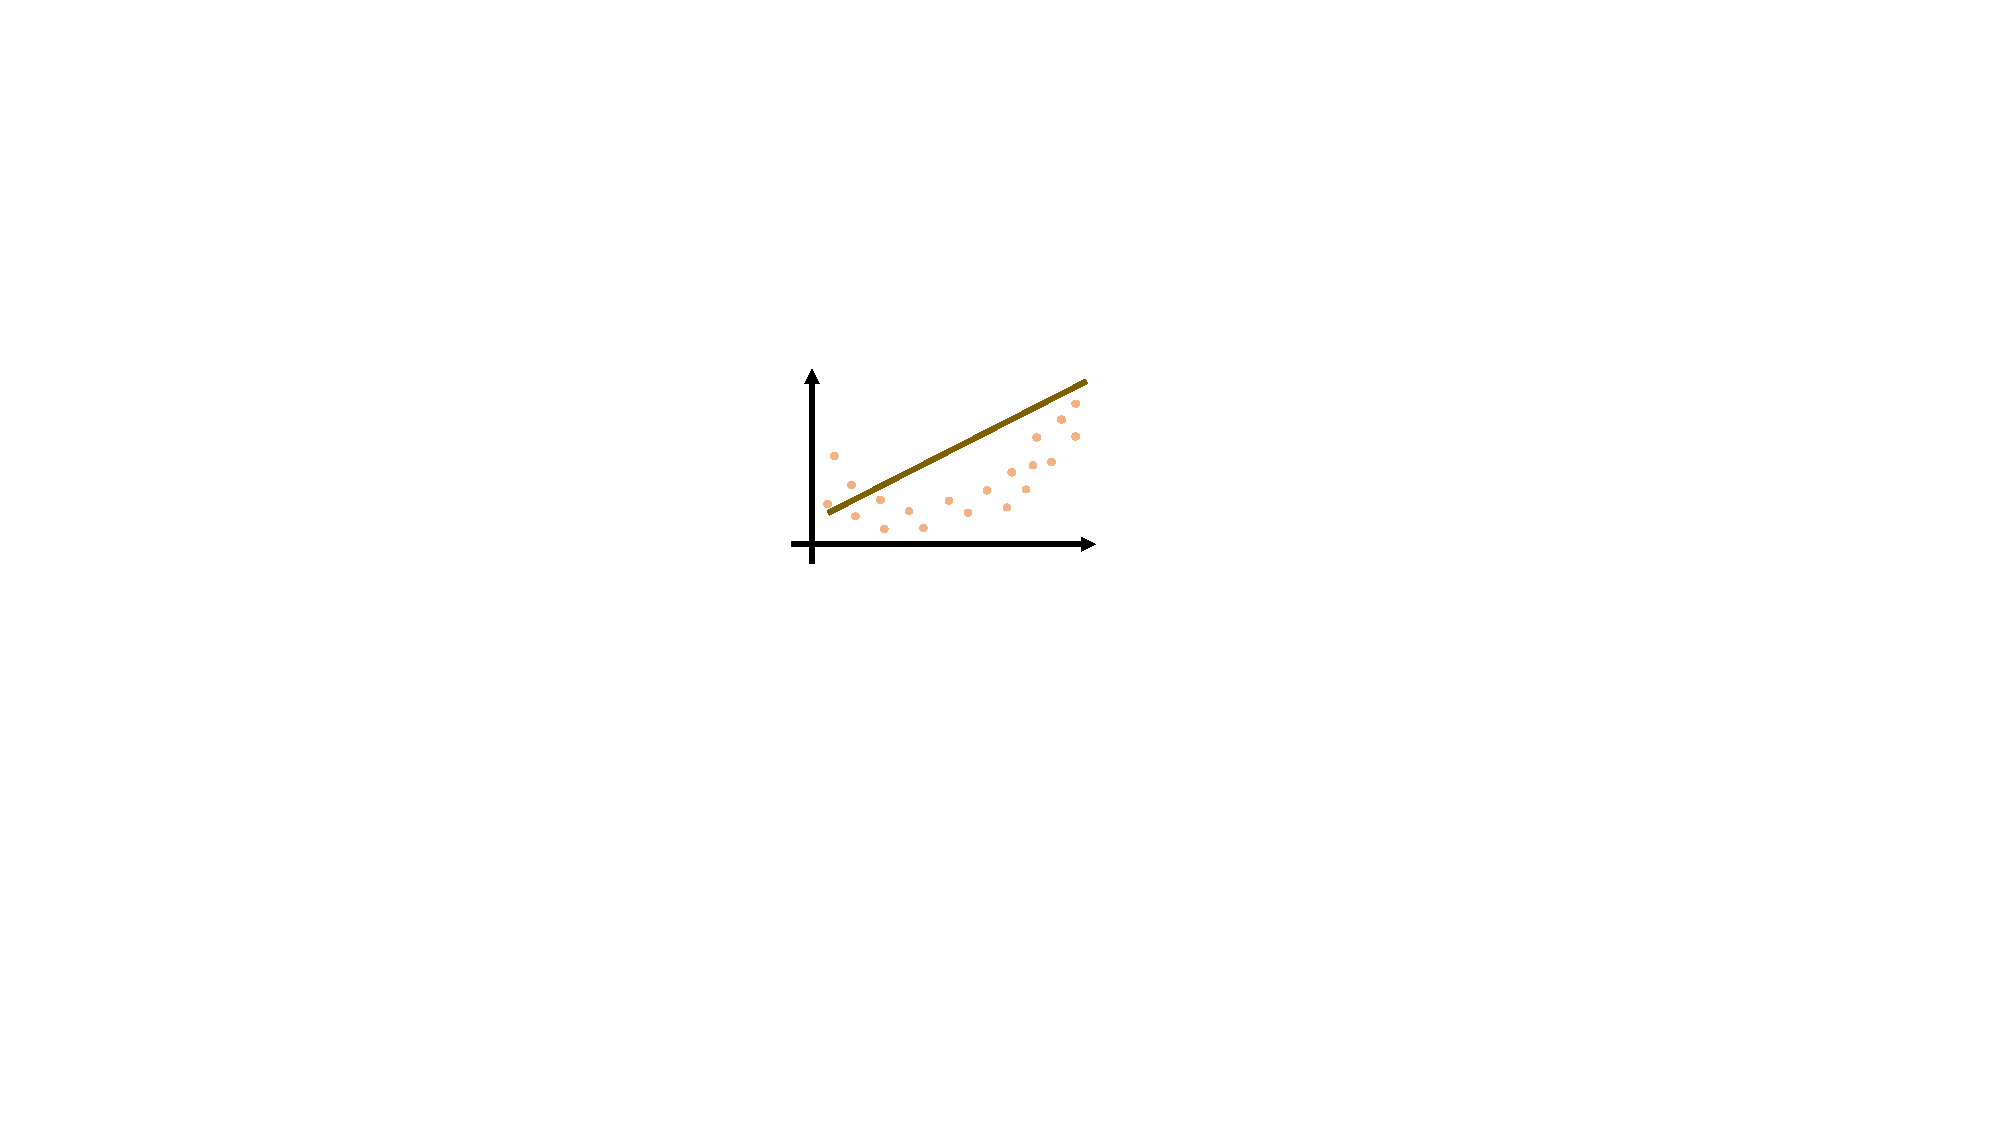
\includegraphics[scale=0.75]{high_bias.pdf}
        \end{minipage}
    }%
    \subfigure[Just Right]{
        \begin{minipage}[t]{0.3\textwidth}
            \centering
            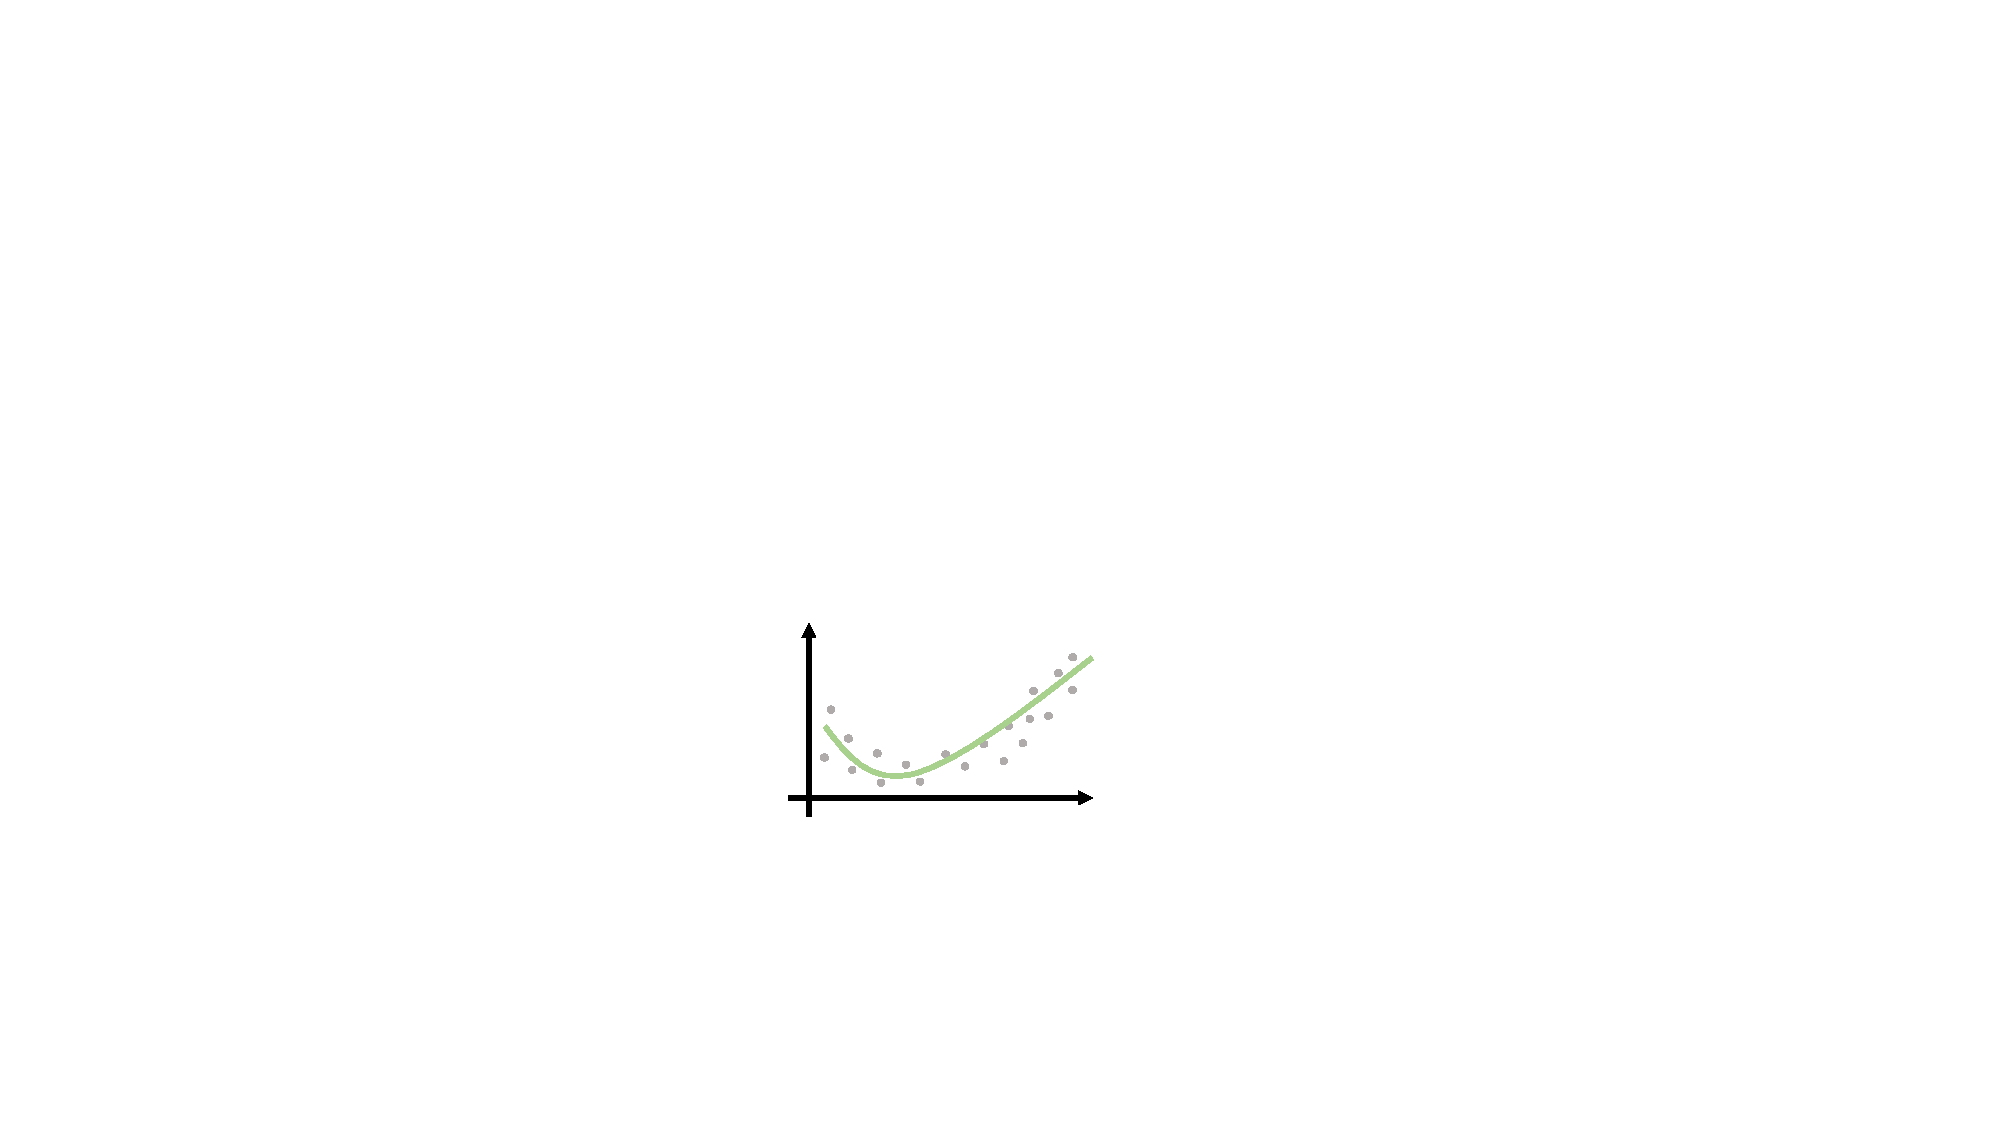
\includegraphics[scale=0.75]{just_right.pdf}
        \end{minipage}
    }%
    \subfigure[High Variance]{
        \begin{minipage}[t]{0.3\textwidth}
            \centering
            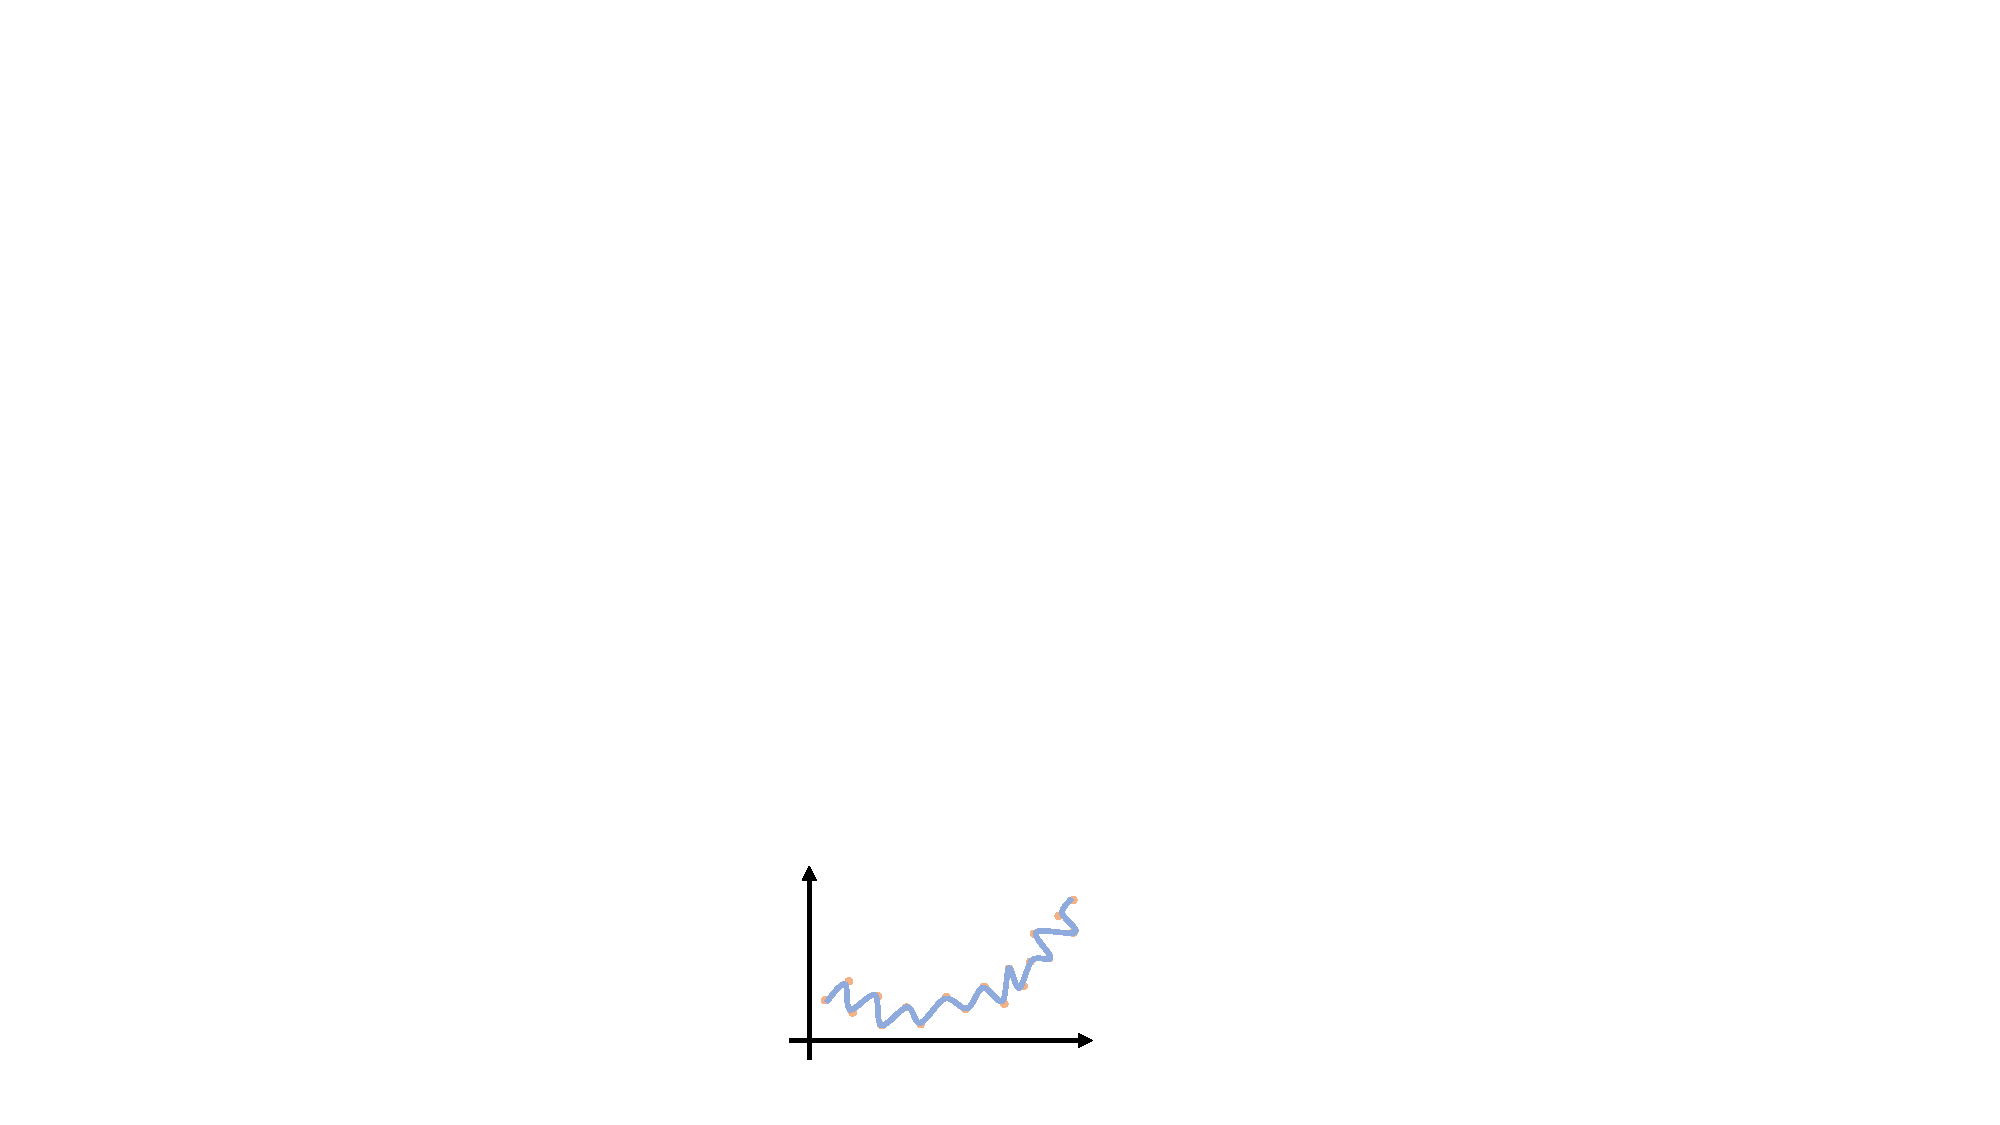
\includegraphics[scale=0.75]{high_variance.pdf}
        \end{minipage}
    }%
    \centering
    \caption{Bias and Variance}
    \label{fig:bias-variance}
\end{figure}

\textbf{高偏差(High bias)}通常表示模型欠拟合,即模型的复杂度不够,无法拟合数据。这可以体现在模型在训练集上的误差和在开发集上的误差都很大,且二者之间的差距不大。
而\textbf{高方差(High variance)}通常表示模型过拟合,即模型的复杂度过高,导致模型过于敏感,无法泛化。这可以体现在模型在训练集上的误差很小,但在开发集上的误差很大。
若高偏差和高方差同时存在,则会体现在模型在训练集上的误差和在开发集上的误差都很大,且开发集上的误差明显大于训练集上的误差。

当我们发现模型的偏差很大时,可以尝试使用更大的网络、训练更长的时间、使用更好的优化算法等来提高模型的复杂度,从而减小偏差。
而当我们发现模型的方差很大时,可以尝试使用更多的数据、使用正则化、使用dropout等来减小模型的复杂度,从而减小方差。

%%%%
\subsection{Regularization}
